% ==============================================================
% CAPÍTULO 4 — MEIO AMBIENTE
% ==============================================================

\chapter{Meio Ambiente}
\label{cap:meio-ambiente}

\section{Mercado de Healthtechs e Fintechs}

\subsection{O ecossistema brasileiro de healthtechs}

O setor de saúde vem sendo reconfigurado pelas healthtechs, startups que combinam tecnologia e saúde para reduzir custos, ampliar acesso e melhorar a experiência de pacientes e profissionais. O Brasil lidera esse movimento na América Latina, concentrando 64,8\% das healthtechs investidas na região. Em 2025, o setor de saúde ultrapassou o de fintechs e tornou-se a segunda maior vertical do ecossistema de startups do país, com 9,4\% das empresas ativas.

O capital aportado tem se mostrado mais seletivo: em 2024, os negócios envolvendo startups de saúde movimentaram R\$~799 milhões, 24\% a menos do que em 2023, mas com 38\% mais startups conseguindo captar. Os investidores priorizam empresas com produto validado e múltiplas fontes de receita, o que favorece o perfil da Capim \cite{distrito2024healthtech, abstartups2025}.

\subsection{O ecossistema brasileiro de fintechs}

O Brasil também lidera o ecossistema de fintechs latino-americano, com 1.706 empresas em operação de um total de 3.500 na região. O mercado atingiu USD~4,73 bilhões em 2024, com projeção de USD~17,58 bilhões até 2033, crescimento anual de 15,70\%. O volume de crédito concedido por fintechs cresceu 68\% em 2024, chegando a R\$~35,5 bilhões \cite{distrito2025fintech, imarc2024, abcdpwc2024}.

A Capim atua no cruzamento desses dois ecossistemas, sendo uma healthtech com componente fintech embarcado, que integra gestão de clínica via SaaS, parcelamento ao paciente via BNPL e adquirência via POS.

\subsection{O mercado odontológico brasileiro}

O Brasil possui 449 mil cirurgiões-dentistas registrados, 20\% dos profissionais do mundo. O setor movimentou US\$~4,6 bilhões em 2022, com projeção de US\$~6,9 bilhões em 2030, crescendo 5,2\% ao ano.

A demanda é majoritariamente privada: 68\% dos brasileiros visitaram um dentista no último ano, mas apenas 23\% dos atendimentos foram pelo SUS. Os planos odontológicos alcançaram 34,34 milhões de beneficiários em novembro de 2024, crescimento de 6,83\% no período \cite{cfo2024, grandviewresearch2023, ans2024}. As clínicas, unidade central do modelo da Capim, faturam entre R\$~20 mil e R\$~35 mil mensais no caso de consultórios individuais, entre R\$~40 mil e R\$~70 mil no caso de clínicas de médio porte, e acima de R\$~100 mil no caso de clínicas maiores. O subsetor de healthtechs especializadas em odontologia ainda é pequeno, com estimativa de 30 a 60 empresas relevantes no Brasil, a maioria sem produto completo ou escala operacional -- o que representa uma oportunidade de consolidação.

\subsection{TAM, SAM e SOM da Capim}

A Figura~\ref{fig:tam-sam-som} ilustra a redução sucessiva do mercado endereçável; as premissas de cada nível estão detalhadas a seguir.

\begin{figure}[h]
  \caption{Funil TAM, SAM e SOM da Capim}
  \label{fig:tam-sam-som}
  \centering
  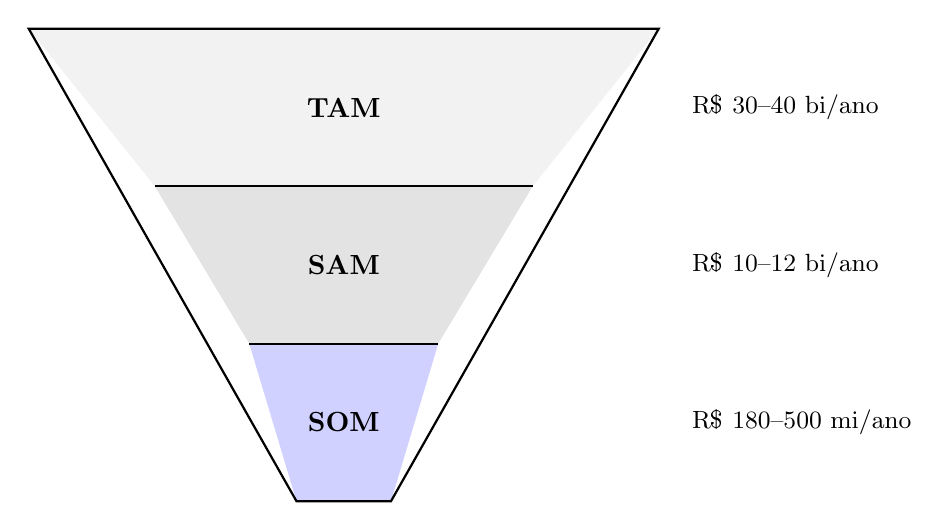
\begin{tikzpicture}[font=\small]
    \fill[gray!10]  (-4,6) -- (4,6)  -- (2.4,4) -- (-2.4,4) -- cycle;
    \fill[gray!22]  (-2.4,4) -- (2.4,4) -- (1.2,2) -- (-1.2,2) -- cycle;
    \fill[blue!18]  (-1.2,2) -- (1.2,2) -- (0.6,0) -- (-0.6,0) -- cycle;
    \draw[thick] (-4,6) -- (4,6) -- (0.6,0) -- (-0.6,0) -- cycle;
    \draw[thick] (-2.4,4) -- (2.4,4);
    \draw[thick] (-1.2,2) -- (1.2,2);
    \node[font=\bfseries] at (0,5) {TAM};
    \node[anchor=west] at (4.3,5) {R\$~30--40 bi/ano};
    \node[font=\bfseries] at (0,3) {SAM};
    \node[anchor=west] at (4.3,3) {R\$~10--12 bi/ano};
    \node[font=\bfseries] at (0,1) {SOM};
    \node[anchor=west] at (4.3,1) {R\$~180--500 mi/ano};
  \end{tikzpicture}
  \legend{Fonte: estimativas dos autores a partir de dados secundários -- a confirmar.}
\end{figure}

O TAM é o mercado odontológico privado brasileiro como um todo. O SAM considera apenas as clínicas privadas independentes com perfil de digitalização compatível com os produtos da Capim (excluindo SUS e grandes redes com sistemas próprios), partindo de um universo estimado de 80 a 100 mil clínicas ativas com ticket médio mensal entre R\$~1.500 e R\$~10.000. O SOM considera uma penetração de 3\% a 5\% dessas clínicas em cinco anos -- entre 2.500 e 5.000 clínicas ativas, ticket médio ponderado entre R\$~6.000 e R\$~10.000 mensais --, meta plausível dado o crescimento atual da base e o aumento de ticket proporcionado pelo produto POS.

A Capim opera em um setor estruturalmente atraente pelo tamanho do mercado odontológico privado, pelo momentum do ecossistema brasileiro de healthtechs e pela convergência com o mercado de fintechs. Esse posicionamento no cruzamento dos dois ecossistemas amplia o SAM endereçável em relação a concorrentes que atuam em apenas um vetor -- software, parcelamento ou maquininha isoladamente.

\section{Principais Concorrentes}

A Capim compete em três frentes simultâneas, pois seu modelo une software de gestão (SaaS), parcelamento ao paciente (BNPL) e adquirência (POS). Isso significa que a empresa não enfrenta um único concorrente direto que replique essa combinação, mas diferentes competidores em cada camada do produto.

\subsection{Concorrentes no SaaS de gestão odontológica}

O mercado brasileiro de software para clínicas odontológicas é fragmentado, com alguns players consolidados e muitos sistemas de nicho. Os dois líderes são o Simples Dental e o Clinicorp. O Simples Dental é descrito como o maior software odontológico da América Latina, com mais de 60 mil dentistas cadastrados no Brasil, diferencial de interface simples e automação de comunicação via WhatsApp, mais forte em clínicas pequenas e médias. O Clinicorp se posiciona como o sistema mais completo do mercado, com módulos de CRM, funil de vendas, gestão financeira avançada, controle multiunidade e integração com IA para análise de dados, atendendo mais de 57 mil usuários ativos, voltado a clínicas estruturadas e redes com múltiplas unidades. Outros players relevantes são o Dental Office, voltado a clínicas de médio porte com foco em controle financeiro e agendamento, e o Codental, mais direcionado a consultórios individuais.

\subsection{Concorrentes no BNPL e adquirência}

O Simples Dental oferece integração com a Parcela Mais, fintech especializada em crédito para saúde. O Clinicorp oferece funcionalidade similar por meio do Clinipay, sua solução própria de pagamentos. Outras fintechs de crédito para saúde, como KonsigaPay, EFIC e Finnsaúde, também atuam nesse espaço, mas sem integração nativa com software de gestão. Existem ainda concorrentes generalistas em BNPL, como Koin e Qista, sem produto especializado para odontologia. No produto de maquininha, a Capim compete com players generalistas de adquirência como Stone, PagSeguro e InfinitePay, que têm vantagens estruturais de escala e taxas, mas não têm especialização em odontologia nem integração com a rotina clínica.

\subsection{Síntese competitiva}

% TODO(equipe): complementar esta seção com uma análise de concorrentes nos moldes da aula 3 (material a inserir por quem participou da aula).
A Tabela~\ref{tab:concorrentes} resume o posicionamento dos principais players nas três camadas de produto.

\begin{table}[h]
  \centering
  \caption{Comparativo de concorrentes por camada de produto}
  \label{tab:concorrentes}
  \begin{tabular}{lccc}
    \toprule
    \textbf{Empresa} & \textbf{SaaS de gestão} & \textbf{BNPL nativo} & \textbf{POS integrado} \\
    \midrule
    Capim            & Sim & Sim            & Sim            \\
    Simples Dental   & Sim & Via parceiro   & Não            \\
    Clinicorp        & Sim & Via Clinipay   & Via Clinipay   \\
    Dental Office    & Sim & Não            & Não            \\
    Stone / PagSeguro& Não & Não            & Sim            \\
    \bottomrule
  \end{tabular}
  \legend{Fonte: elaborado pelos autores a partir de dados secundários (2026).}
\end{table}

Nenhum concorrente combina os três produtos com a profundidade da Capim. O Clinicorp é o player mais próximo em abrangência, mas seu produto financeiro funciona como uma camada adicional sobre o software, sem análise de crédito proprietária e sem exposição direta ao risco de inadimplência como faz a Capim.

\section{Posicionamento da Capim}

A Capim se posiciona como a única plataforma do mercado brasileiro que oferece, de forma nativa e integrada, gestão de clínica, parcelamento ao paciente e adquirência. Fundada em 2021 por Marcelo Lutz e Roberto Biselli, a empresa se define como um ERP especializado em odontologia, com camada financeira embarcada. Em fevereiro de 2025, captou uma Série A de R\$~132 milhões liderada por Valor Capital e QED Investors, com participação de ONE.VC, Canary, NXTP, Endeavor, Saison e Actyus -- este último conduzido por Sérgio Furio, CEO da Creditas. Em 2024, a receita triplicou e a base de clínicas passou a casa dos 6 mil, com o objetivo declarado de alcançar 10 mil clínicas ativas. \footnote{Dados de fundação, captação e investidores são informações institucionais/de mercado, não relatadas pelo entrevistado -- a equipe deve confirmar a exatidão e a fonte antes da entrega final.}

\subsection{Principal diferencial}

O diferencial central da Capim é assumir o risco de crédito do paciente diretamente, em vez de apenas intermediar a transação. Quando um financiamento é fechado, a clínica recebe à vista e a Capim fica responsável por toda a cobrança e pela inadimplência, sem direito de regresso contra a clínica em tratamentos já executados. Isso muda a economia da clínica, que deixa de carregar carteira de recebíveis e ganha previsibilidade de caixa, e cria para a Capim um ativo financeiro proprietário, baseado em dados próprios de comportamento de pagamento que se acumulam a cada operação.

A combinação SaaS, BNPL e POS no mesmo ambiente gera três efeitos competitivos importantes: eleva o ticket médio por clínica (mensalidade, taxa sobre TPV e spread sobre parcelamento); aumenta o custo de troca, já que sair da Capim implica trocar três fornecedores simultaneamente; e cria um ciclo de dados próprio, no qual o comportamento financeiro de pacientes e clínicas alimenta o motor de crédito e o produto de gestão -- loop que concorrentes de vetor único não conseguem replicar.

\subsection{Tecnologias e capacidades técnicas}

A plataforma é 100\% \textit{online}, acessível por celular, tablet ou computador, e segue os requisitos da LGPD. Suas principais capacidades técnicas são: um motor de análise de crédito proprietário, que consulta Serasa e Boa Vista e gera um Score Capim próprio em tempo real; um sistema de parcelamento em até 36 vezes, com juros aproximadamente 50\% menores que os praticados por bancos tradicionais para crédito ao consumidor; uma régua de cobrança automatizada via WhatsApp, e-mail e ligação telefônica; uma camada de gestão clínica completa, integrada ao motor financeiro; um terminal POS proprietário, lançado a partir de 2025 com o capital da Série A; e uma camada de inteligência artificial em desenvolvimento, voltada à automação administrativa e à geração de alertas e sugestões para o gestor da clínica.

A Capim ocupa, assim, uma posição estratégica no cruzamento entre healthtech e fintech, em um nicho historicamente subatendido por sistemas de saúde de uso geral. Os capítulos seguintes tratam dos desafios de governar a inovação dentro dessa posição.
